\section{Discussion}
We  note at the outset that the sensitivity analysis investigates the numerical model rather than the physiological one. However, since the numerical model has been validated with experimental data, \todo[inline]{need a reference} the results should indicate areas (and therefore parameters) of importance for physiologists and modellers. The integration times $t_1,t_2$ are the start and end of neuronal stimulation. Decreasing or increasing these time does not significantly alter the ranking of the parameters. We discuss below results for each QoI individually. 


\subsection{ECS $K^+_{mean}$}
It is interesting to note for this particular quantity of interest that the two top most important parameters are associated not with a \pot channel but the persistent \na channel, NaP.  The neuron model used in this analysis was developed from the work of Kager et al \cite{Kager2000a} and Chang et al \cite{Chang2013}.
The differential equation governing $m_4$,  the activation variable for the NaP channel, is given by 
\begin{eqnarray}
\frac{d m_4}{dt} = m_{4 \alpha}(1 - m_4) - (m_{4\beta} \, m_4), \label{eqn:m4alpha}
\end{eqnarray}
with $\displaystyle m_{4 \alpha}= \frac{1}{6(1 + \exp(-((c_1 v_d) + c_2)))}$ and $m_{4 \beta} = m4_{\alpha} \exp(-((c_1 v_d) + c_2))$; the nominal parameter values are $c_1=0.143$ and $c_2=5.67$.

The inactivation of the NaP channel is very small compared to activation and therefore these parameters make little impact on the extracellular \pot. 
Scatter plots for the mean of \pot in the  ECS against the parameter value for each of the 2 most important parameters ranging over $\pm 10\%$  are shown in Figure \ref{fig:scatter}.  For each parameter, there is a linear trend where increasing the parameter yields either an increase or decrease in the \pot ECS. No single parameter will be able to accurately predict the extracellular \pot, but the results indicate a clear trend. The characteristic time for the activation variable for the NaP channel is defined as $\tau=\frac{1}{m_{4 \alpha}+m_{4 \beta}}$ which by using equation (\ref{eqn:m4alpha}) is constant (6 ms). The scatter plots also indicate this definition. These results indicate therefore that in order to either reduce or increase the extracellular \pot a variation of $\pm 10 \%$ can induce an approximate variation of 15 $\%$. We should note that these results do not take into account the spatial buffering carried out by the astrocytic syncytium which may have a significantly greater effect on the extracellular \pot. 
\todo[inline]{reference here of work by Kenny as well as \cite{Bellot-Saez2017} and possibly others}
\begin{figure}
\centering
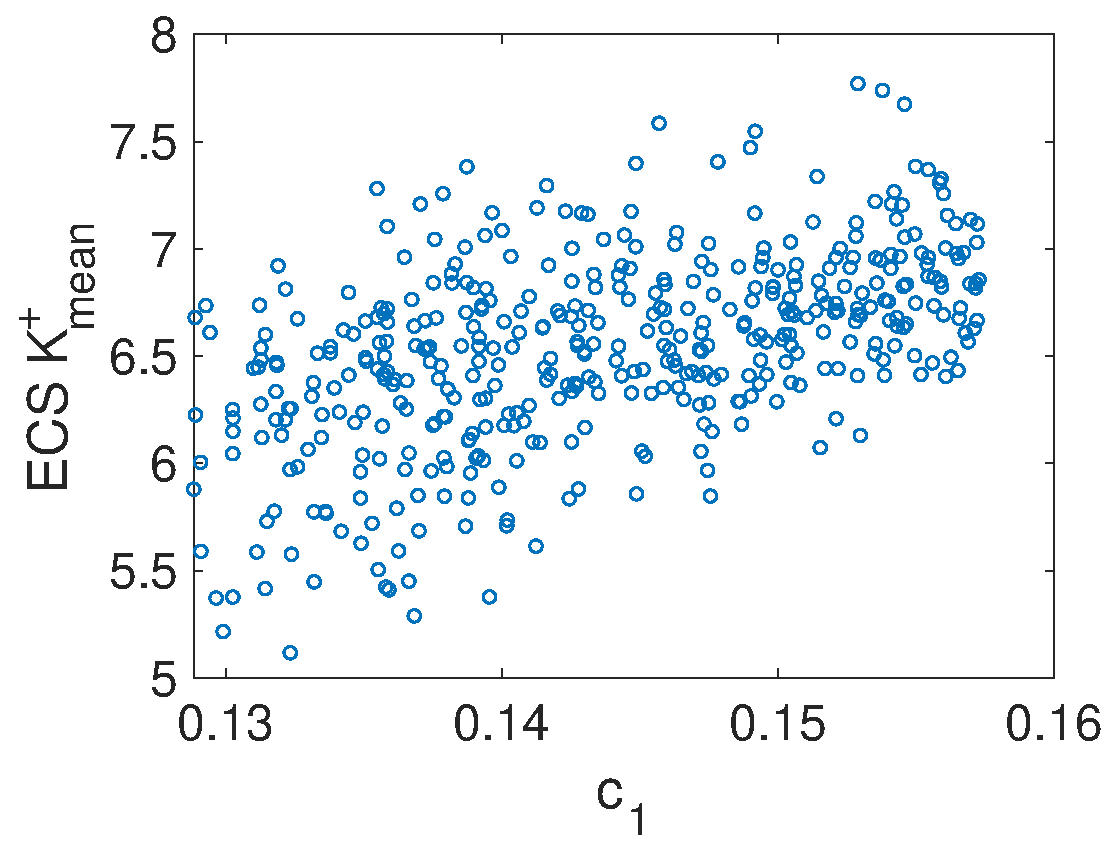
\includegraphics[width=0.49\linewidth]{Figures/Scatter_62_K_ECS}
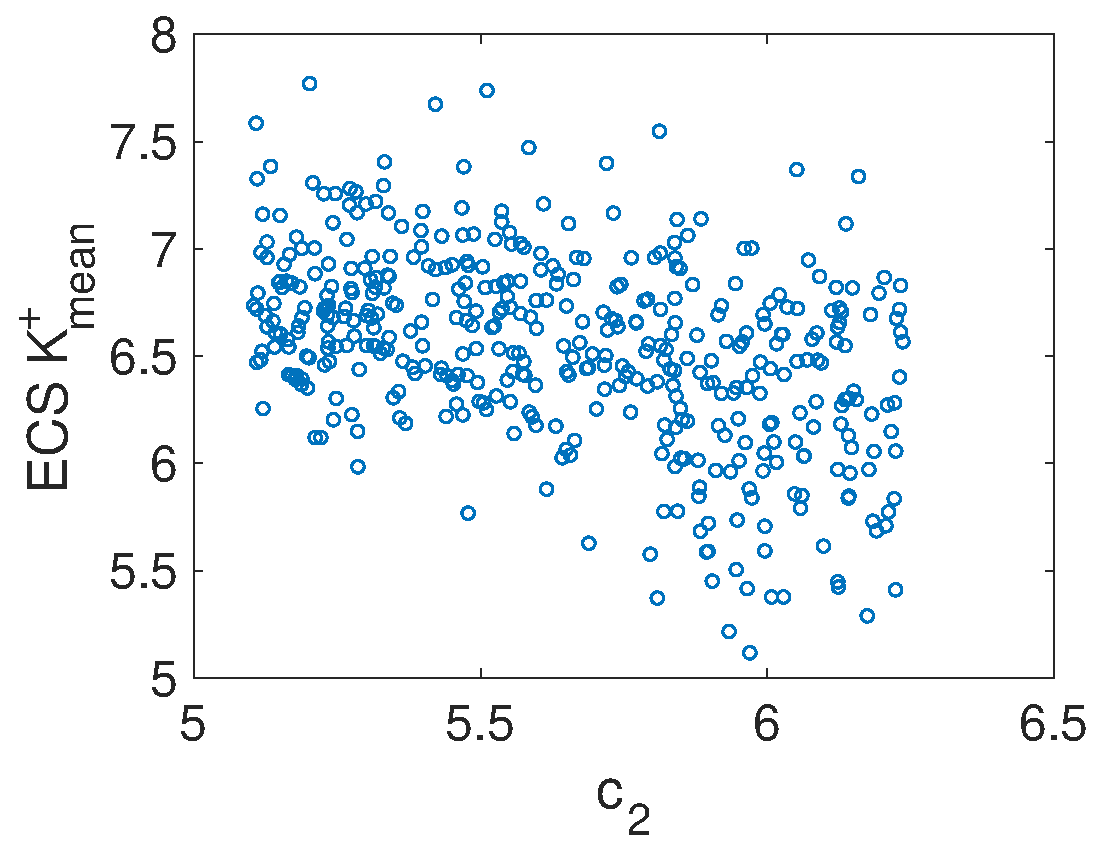
\includegraphics[width=0.49\linewidth]{Figures/Scatter_63_K_ECS}
\caption{Left: scatter plot of $c_1$ (parameter index 62) and ECS $K^+_{mean}$; right: scatter plot of $c_2$ (parameter index 63) and ECS $K^+_{mean}$.}
\label{fig:scatter}
\end{figure}
The main driver for \pot in the extracellular space is the \pot \na ATP-ase pump which has the general form given by (in the dendrite)  
\begin{eqnarray}\label{eqn:ATP-ase}
\frac{Na_d^3}{\left( Na_d+Na_{d init}\right)^3}\frac{K^{2}_e}{\left( K^+_e +K^+_{e init}\right) ^2}
\end{eqnarray}
The ATP-ase pumps out \na and in \pot in the ratio of 3 to 2, hence the \na in the dentrite has a large effect on the extracellular \pot as seen in equation (\ref{eqn:ATP-ase}) and strengthens the result that the NaP channel has the most effect on the \pot. One could have expected the NaT (transient \na) channel to be prominent however, this has a fast inactivation variable and although produces a larger flux does so over a shorter time.  
\subsection{Volumetric Flow Rate}
In the presented model the main pathway for neurovascular coupling is that of the \pot pathway. Here the astrocyte takes up \pot from the synaptic cleft and provides an efflux into the perivascular space (PVS) via the BK channel. The smooth muscle cell detects this increase in PVS \pot and through the inwardly rectifying channel ($K_{IR}$) hypopolarises the SMC , shutting off the voltage mediated \ca channel.  \ca is therefore reduced and the SMC dilates. As stated in the Results section (indicated by equation (\ref{eq:gkir})) the most important parameter is that of the ``shift" parameter $z_4$ in the $K_{IR}$ conductance determining the magnitude of ion flux per unit change in the membrane potential away from the equilibrium (Nernst potential).  Compared to the other parameters in defining the $K_{IR}$ conductance $z_4$ is large with a value of 12.6 compared to $z_3=4.2 \times 10^{4} \mu M^{-1}$ and $z_5 = -7.4 \times mV^{-1}$. Hence, for constant membrane potential and \pot,   variations in $z_4$ produce exponentially large variations in the $K_{IR}$ channel conductance allowing substantial efflux of \ca from the SMC and a dilation of the vessel ($\frac{dR}{dt}> 0$). \\

The second most dominant parameter is the power index for the cytosolic SMC \ca which mediates the four state latch model of Hai and Murphy \cite{Hai1988}, in particular the rate of phosphorylation of  myosin and the actin-myosin complex.  Variations in \ca as predominantly dictated by the $K_{IR}$ channel will therefore have a direct effect on the dilation/contraction properties of the SMC and hence the perfusing vessel radius.  
The remaining three parameters have significantlly lower Total Sobol indices and therefore play only a very small part in the quantity of interest.\\
 
\subsection{$[AM+AM_p]_{min}$}
For this particular QoI we see similar parameters appearing which is to be expected given the strong relationship between the radius dilation/contraction phenomenon and the total quantity of actin/myosin complex and its phosphorylated compliment. In fact this QoI serves as a test of the statistical mechanism in that the only two non-repeating variables between the radius QoI and the actin/myson complex is the leak conductance GKi and $z_3$ which as noted above have very little effect. 
